\documentclass[11pt]{article}

\usepackage[margin=.75in]{geometry}
\usepackage{amsmath}
\usepackage{array}
\usepackage{booktabs}
\usepackage{graphicx}
\usepackage{hyperref}
\usepackage{tabularx}
\usepackage{xcolor}
\usepackage{fvextra}

\hypersetup{
    colorlinks=true,
    linkcolor=blue,
    citecolor=blue,
    urlcolor=blue
}

\newcommand{\todo}[1]{\textcolor{red}{TODO: #1}}
\DefineVerbatimEnvironment{answerbox}{Verbatim}{breaklines=true,breakanywhere=true,fontsize=\footnotesize}
\newcommand{\placeholderfig}[3]{%
\begin{figure}[t]
    \centering
    \fbox{%
        \begin{minipage}[c][1.45in][c]{0.9\linewidth}
            \centering
            \textbf{#2}\\[0.4em]
            #3
        \end{minipage}%
    }
    \caption{#2. #3}
    \label{#1}
\end{figure}
}

\title{Post-Training Qwen2.5-1.5B with SFT, GRPO, and vLLM Rollouts}
\author{zcm25@mails.tsinghua.edu.cn}
\date{June 2026}

\begin{document}
\maketitle

\begin{abstract}
This report studies a post-training pipeline for \texttt{Qwen/Qwen2.5-1.5B} on mathematical reasoning. I first implement supervised fine-tuning (SFT) on the \texttt{AI-MO/NuminaMath-CoT} subset with \texttt{source = gsm8k}, then implement Group Relative Policy Optimization (GRPO) on GSM8K, and finally explore vLLM rollout acceleration for RL training. The main result is that SFT improves GSM8K accuracy over the base model, while GRPO gives the strongest final performance, reaching 77.03\% GSM8K accuracy and 54.41\% MMLU accuracy.
\end{abstract}

\section{Introduction}
Modern LLM post-training typically combines imitation learning with reinforcement learning. In this project, I build this pipeline from scratch for \texttt{Qwen/Qwen2.5-1.5B}, evaluate the model before and after each stage on GSM8K and MMLU, and investigate whether vLLM rollout generation can make GRPO training more efficient without degrading downstream accuracy.

\paragraph{Main results.}
\begin{itemize}
    \item Step-by-step prompting is already important for the base model, raising GSM8K from 52.31\% with the simple prompt to 67.78\% with the step-by-step prompt. MMLU uses a fixed prompt and achieves 33.29\%.
    \item The best SFT checkpoint reaches 67.93\% GSM8K accuracy and 36.76\% MMLU accuracy.
    \item The best GRPO checkpoint reaches 77.03\% GSM8K accuracy and 54.41\% MMLU accuracy.
    \item vLLM rollout can significantly accelerates training, achieving \(\sim 3\times\) speedup while slightly hurting accuracy.
\end{itemize}

\paragraph{Interesting Observations.}
\begin{itemize}
    \item Adding "Please think step by step" is much more cost-efficient than finetuning. They achieved similar accuracy but prompting requires no training at all.
    \item SFT with and without "please think step by step" prompts achieves similar \texttt{GSM8K} evaluation result, but thinking step by step makes the model more robust: avoids accuracy decrease in the \texttt{MMLU} dataset.
    \item GRPO make the model more instruction obediant. It achieves large MMLU gains by simply outputting recognizable choice answers.
    \item Setting max new tokens generated to \(256\) during GRPO pushed the model to use \texttt{\#\#\#<answer>} rather than \verb|\boxed{<answer>}|, and produce more concise reasoning without much drop in accuracy.
    \item vLLM speeds up inference during evaluation almost \(20\times\) compared to huggingface generate.
    \item Qwen really likes to say "You are an AI assistant that helps people find information ..."
\end{itemize}

\begin{table}[t]
\centering
\caption{Best evaluation results.}
\label{tab:headline-results}
\begin{tabular}{l r r}
\toprule
Stage & GSM8K & MMLU \\
\midrule
Base & 52.31\% & 33.29\% \\
Base + step-by-step prompt & 67.78\% & 33.29\% \\
SFT & 67.93\% & 36.76\% \\
GRPO & 77.03\% & 54.41\% \\
\bottomrule
\end{tabular}
\end{table}

\section{Experimental Setup}
\subsection{Model and Data}
The base model is \texttt{Qwen/Qwen2.5-1.5B}. SFT uses \texttt{AI-MO/NuminaMath-CoT} filtered to \texttt{source = gsm8k}. GRPO uses the \texttt{openai/gsm8k} training split for rollouts. Evaluation uses the GSM8K test split and the elementary mathematics, high school mathematics, and college mathematics subsets of the MMLU test split.

\subsection{Evaluation Protocol}
GSM8K is evaluated with both a simple prompt and a step-by-step prompt for base/SFT checkpoints, while GRPO checkpoints are evaluated with the simple GSM8K prompt. 

For GSM8K answer checking, I use the \texttt{math\_verify} package. MMLU uses one fixed generative multiple-choice prompt and is restricted to the elementary mathematics, high school mathematics, and college mathematics subjects. The answer extraction logic is intentionally strict: the evaluator first looks for the last \verb|\boxed{...}| answer, then falls back to final-answer markers such as \texttt{\#\#\#\#}, ``final answer is'', or ``answer is''. The extracted text is stripped of lightweight formatting characters such as dollar signs, backticks, trailing periods, and whitespace. A prediction is counted only if it normalizes to a single choice in \texttt{A}/\texttt{B}/\texttt{C}/\texttt{D} or \texttt{1}/\texttt{2}/\texttt{3}/\texttt{4}, with numbers mapped to letters. The normalized prediction is compared against the gold MMLU label converted from the dataset's class index.

\paragraph{Prompt templates.}
These templates mirror the prompt builders in \texttt{prompts.py} and define the exact model-facing inputs used by SFT, GRPO, and evaluation.

\begin{quote}
\small
\textbf{GSM8K simple}
\begin{answerbox}
Problem:
{problem}

Solution:
\end{answerbox}
\end{quote}

\begin{quote}
\small
\textbf{GSM8K step-by-step}
\begin{answerbox}
Solve the following math problem. Please think step by step, show the reasoning
clearly, and end with the final answer in the form `\boxed{<answer>}`.

Problem:
{problem}

Solution:
\end{answerbox}
\end{quote}

\begin{quote}
\small
\textbf{MMLU}
\begin{answerbox}
The following is a single-choice question about {normalized_subject}. There is
exactly one correct answer.
Choose from exactly four possible final answers: `\boxed{A}`, `\boxed{B}`,
`\boxed{C}`, `\boxed{D}`.
Show your reasoning, then end with exactly one boxed final answer.

Problem: {question}
A. {choice_0}
B. {choice_1}
C. {choice_2}
D. {choice_3}

Solution:
\end{answerbox}
\end{quote}

\subsection{Implementation Summary}
SFT uses next-token prediction with prompt tokens masked out of the loss. GRPO samples grouped completions per prompt, computes GSM8K rewards from normalized numeric answer matching with an optional formatting reward, and optimizes a clipped policy-gradient objective with a reference-model KL penalty. The implementation supports multi-GPU training with DeepSpeed. The vLLM exploration adds rollout backends for HF generation, vLLM server generation, and colocated vLLM generation.

\section{Part 1: Supervised Fine-Tuning}
\subsection{Method}
I train two SFT variants for three epochs: one using a simple prompt template and one using a step-by-step prompt template. This comparison tests whether explicit reasoning-format supervision improves both math accuracy and general MMLU accuracy.

\begin{figure}[t]
\centering
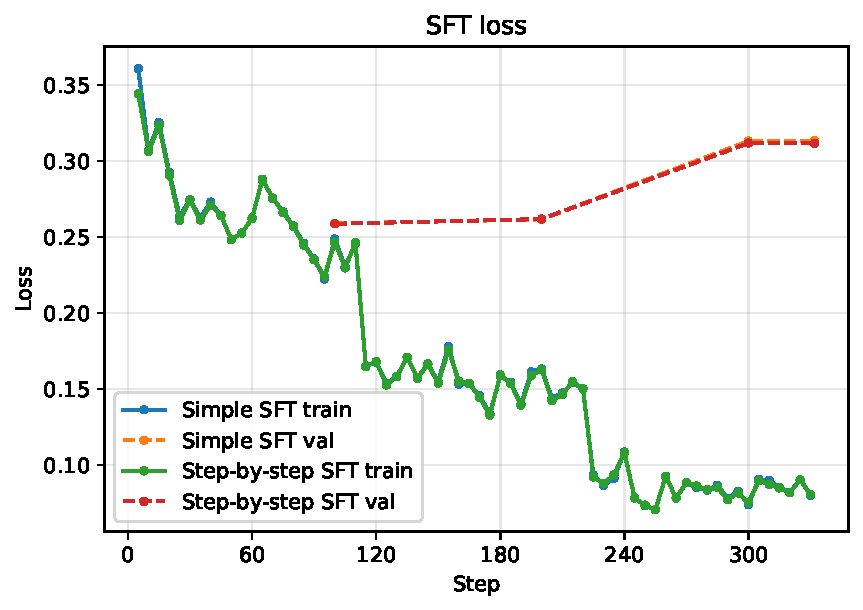
\includegraphics[width=0.78\linewidth]{figures/sft_loss.pdf}
\caption{SFT training and validation loss.}
\label{fig:sft-loss}
\end{figure}

\subsection{Results}
Figure~\ref{fig:sft-loss} shows the SFT training and validation loss curves for the simple and step-by-step prompt variants. Figure~\ref{fig:sft-eval} summarizes the corresponding evaluation accuracy by checkpoint on GSM8K and MMLU. The exact checkpoint-level evaluation numbers are listed in Table~\ref{tab:sft-results}.

\begin{table}[t]
\centering
\caption{Base and SFT evaluation results.}
\label{tab:sft-results}
\begin{tabularx}{\linewidth}{l l r r r}
\toprule
Stage & Checkpoint & GSM8K simple & GSM8K step-by-step & MMLU \\
\midrule
Base & \texttt{Qwen2.5-1.5B} & 52.31\% & 67.78\% & 33.29\% \\
SFT simple & epoch 1 & 62.93\% & 63.31\% & 18.18\% \\
SFT simple & epoch 2 & 66.11\% & 66.72\% & 21.26\% \\
SFT simple & epoch 3 & 66.72\% & 67.02\% & 24.73\% \\
SFT step-by-step & epoch 1 & 62.70\% & 63.46\% & 25.00\% \\
SFT step-by-step & epoch 2 & \textbf{67.93\%} & \textbf{67.70\%} & \textbf{36.76\%} \\
SFT step-by-step & epoch 3 & 66.94\% & 66.34\% & 34.76\% \\
\bottomrule
\end{tabularx}
\end{table}

\begin{figure}[t]
\centering
\begin{minipage}{0.49\linewidth}
\centering
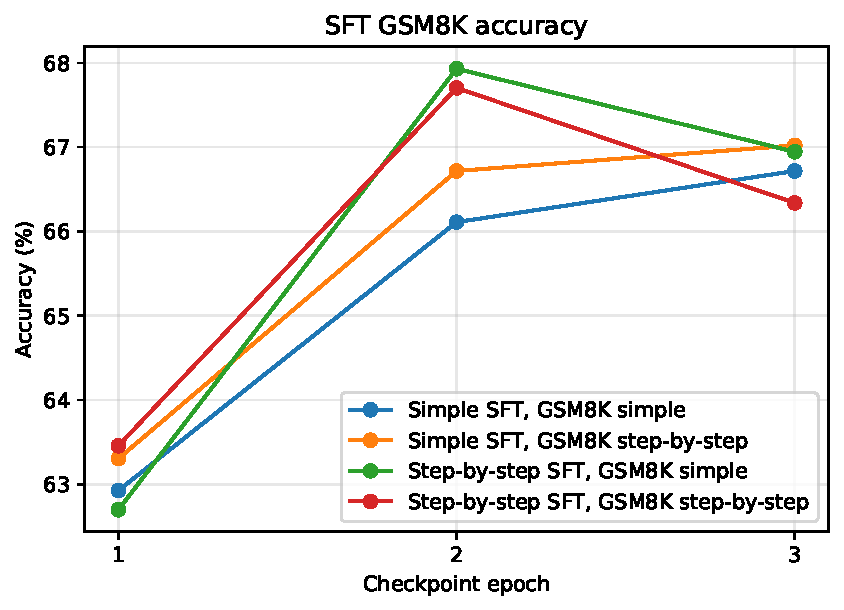
\includegraphics[width=\linewidth]{figures/sft_gsm8k_eval.pdf}
\end{minipage}\hfill
\begin{minipage}{0.49\linewidth}
\centering
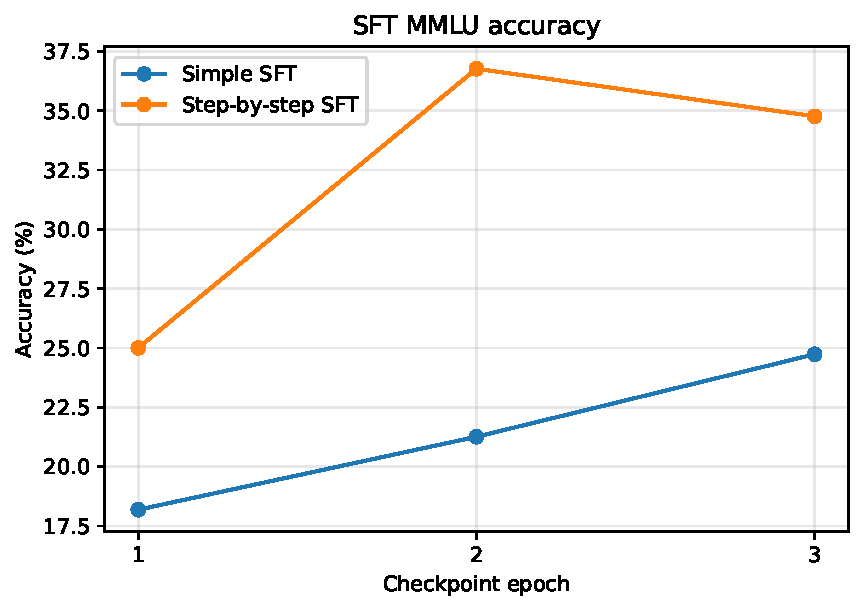
\includegraphics[width=\linewidth]{figures/sft_mmlu_eval.pdf}
\end{minipage}
\caption{SFT evaluation accuracy by checkpoint epoch. Left: GSM8K. Right: MMLU.}
\label{fig:sft-eval}
\end{figure}

\subsection{Observations}
First, prompting the base model to think step by step is already comparable with the best SFT checkpoint on GSM8K. As shown in Table~\ref{tab:sft-results}, the base model reaches 67.78\% GSM8K accuracy with the step-by-step prompt, while the best SFT checkpoint reaches 67.93\% with the simple GSM8K prompt and 67.70\% with the step-by-step prompt. This means a prompt-only intervention nearly matches the best supervised checkpoint in this setting.

Second, the SFT run trained with the step-by-step prompt generally achieves higher MMLU accuracy than the plain-prompt SFT run, supporting the robustness observation in Section~1. Across epochs 1--3, step-by-step SFT obtains 25.00\%, 36.76\%, and 34.76\% MMLU accuracy, compared with 18.18\%, 21.26\%, and 24.73\% for plain-prompt SFT. The two SFT variants remain similar on GSM8K, but the step-by-step variant avoids the larger MMLU drop.

\section{Part 2: GRPO}
\subsection{Method}
GRPO is trained from the base \texttt{Qwen/Qwen2.5-1.5B} policy on GSM8K. Each prompt receives a group of \(G\) sampled completions, and rewards are computed from exact normalized numeric answer matching plus a small formatting reward. Following the TRL \texttt{GRPOTrainer} documentation and the GRPO/Dr. GRPO papers \cite{vonwerra2020trl,shao2024deepseekmathpushinglimitsmathematical,liu2025understandingr1zeroliketrainingcritical}, let \(q\) be a prompt, \(o_i\) be the \(i\)-th completion, \(|o_i|\) be its completion-token length, and \(L\) be the configured maximum completion length. For token \(t\), I write the clipped per-token objective as
\[
\ell_{i,t} =
\min\!\left(
    r_{i,t}(\theta)\hat{A}_{i,t},
    \operatorname{clip}\!\left(r_{i,t}(\theta), 1-\epsilon, 1+\epsilon\right)\hat{A}_{i,t}
\right)
- \beta D_{\mathrm{KL}}\!\left[\pi_\theta \,\|\, \pi_{\mathrm{ref}}\right],
\]
where
\[
r_{i,t}(\theta)=
\frac{\pi_\theta(o_{i,t}\mid q,o_{i,<t})}
{\pi_{\theta_{\mathrm{old}}}(o_{i,t}\mid q,o_{i,<t})}.
\]
The original GRPO loss averages each completion by its own length and then averages across the group:
\[
\mathcal{L}_{\mathrm{GRPO}}(\theta)
=
-\frac{1}{G}\sum_{i=1}^{G}\frac{1}{|o_i|}
\sum_{t=1}^{|o_i|}\ell_{i,t}.
\]
Dr. GRPO changes only the normalization, replacing the response-length denominator with the constant \(L\), which TRL recommends setting to \texttt{max\_completion\_length}:
\[
\mathcal{L}_{\mathrm{Dr.\ GRPO}}(\theta)
=
-\frac{1}{LG}\sum_{i=1}^{G}\sum_{t=1}^{|o_i|}\ell_{i,t}.
\]
This removes the response-length bias introduced by normalizing each sampled response by its own length. In this project, \(L\) is the rollout \texttt{max\_new\_tokens}; I compare \texttt{loss\_type=grpo} with \texttt{loss\_type=dr\_grpo} and evaluate checkpoints after each epoch.

\begin{figure}[t]
\centering
\begin{minipage}{0.49\linewidth}
\centering
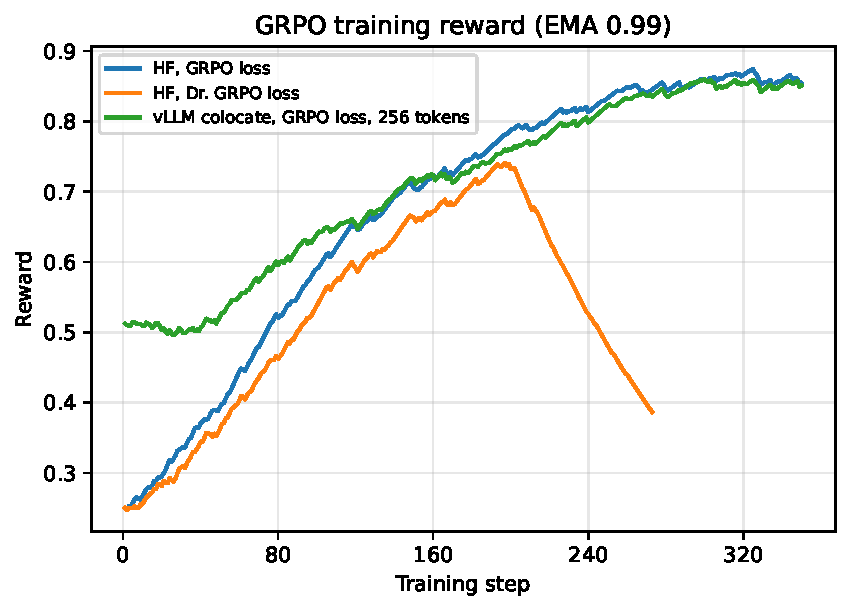
\includegraphics[width=\linewidth]{figures/grpo_reward.pdf}
\end{minipage}\hfill
\begin{minipage}{0.49\linewidth}
\centering
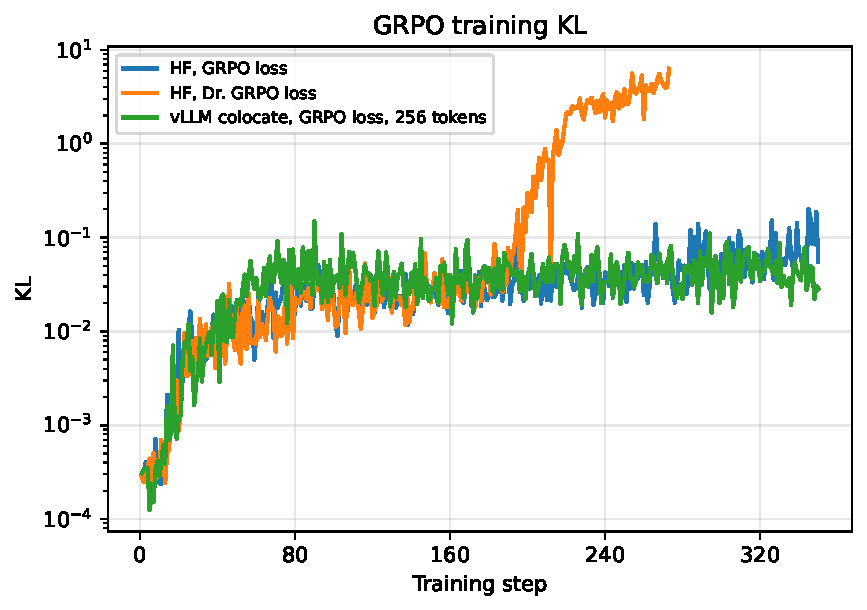
\includegraphics[width=\linewidth]{figures/grpo_kl.pdf}
\end{minipage}
\caption{GRPO training curves for the selected HF GRPO, HF Dr. GRPO, and 256-token colocated vLLM GRPO runs. Left: reward smoothed with EMA 0.99. Right: KL on a log y-axis.}
\label{fig:grpo-training}
\end{figure}

\subsection{Results}
Figure~\ref{fig:grpo-training} summarizes the GRPO reward and KL training dynamics for the selected runs, Figure~\ref{fig:grpo-eval-by-epoch} shows the corresponding GSM8K and MMLU checkpoint evaluation curves, and Table~\ref{tab:grpo-variants} reports the selected final checkpoint results. The \texttt{grpo\_vllm\_colocate\_3epoch\_grpo\_256} run means using vllm colocate as backend, GRPO loss, and \texttt{max\_new\_tokens} during training generation set to 256 instead of default 512.

\begin{table}[t]
\centering
\caption{Selected GRPO variants. Use this table to discuss algorithm and backend sensitivity without turning the main text into a run inventory.}
\label{tab:grpo-variants}
\small
\begin{tabularx}{\linewidth}{X l l r r}
\toprule
Run family & Backend & Loss & GSM8K simple & MMLU \\
\midrule
\texttt{grpo\_hf\_3epoch\_grpo} epoch 2 & HF & GRPO & 77.03\% & 50.13\% \\
\texttt{grpo\_vllm\_server\_pynccl} epoch 3 & vLLM server & GRPO & 76.50\% & 53.21\% \\
\texttt{grpo\_vllm\_server\_tmp} epoch 3 & vLLM server & GRPO & \textbf{77.03\%} & 54.41\% \\
\texttt{grpo\_vllm\_colocate} epoch 3 & vLLM colocate & GRPO & 75.59\% & 54.68\% \\
\texttt{grpo\_vllm\_colocate\_3epoch\_grpo\_256} epoch 3 & vLLM colocate & GRPO & 74.37\% & 39.71\% \\
\texttt{grpo\_vllm\_server\_pynccl\_dr} epoch 3 & vLLM server & Dr. GRPO & 75.97\% & \textbf{54.81\%} \\
\texttt{grpo\_vllm\_colocate\_dr} epoch 3 & vLLM colocate & Dr. GRPO & 76.19\% & 52.54\% \\
\bottomrule
\end{tabularx}
\end{table}

\begin{figure}[t]
\centering
\begin{minipage}{0.49\linewidth}
\centering
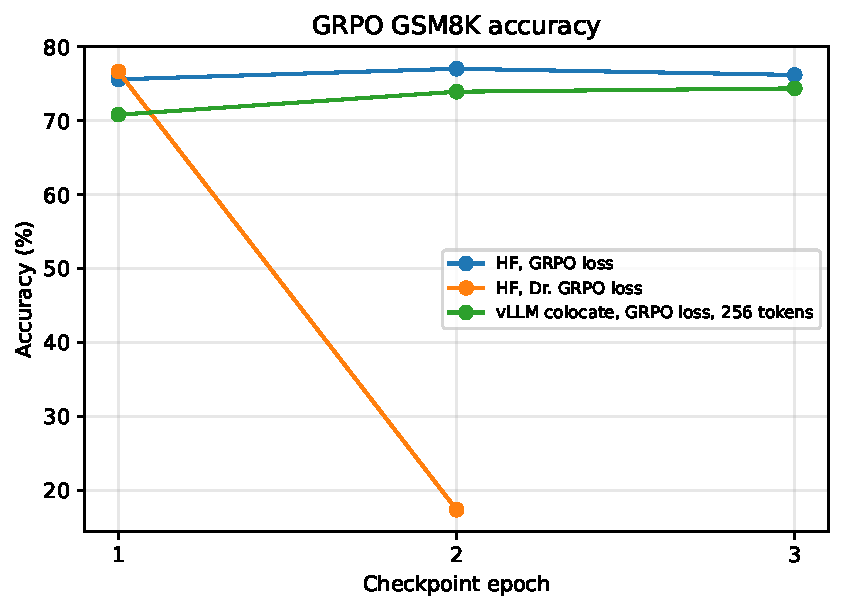
\includegraphics[width=\linewidth]{figures/grpo_gsm8k_eval.pdf}
\end{minipage}\hfill
\begin{minipage}{0.49\linewidth}
\centering
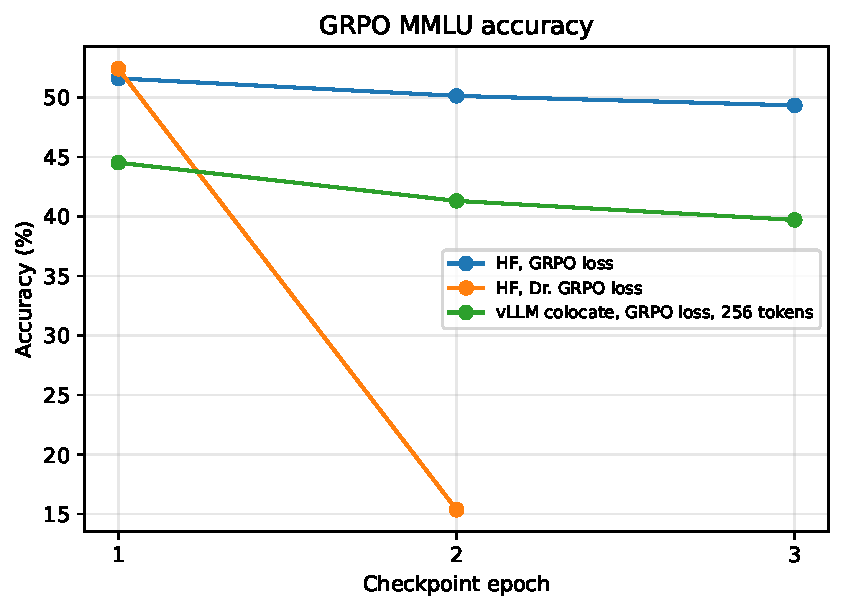
\includegraphics[width=\linewidth]{figures/grpo_mmlu_eval.pdf}
\end{minipage}
\caption{GRPO evaluation accuracy by checkpoint epoch for the selected HF GRPO, HF Dr. GRPO, and 256-token colocated vLLM GRPO runs. Left: GSM8K. Right: MMLU.}
\label{fig:grpo-eval-by-epoch}
\end{figure}

\subsection{Observations}
First, GRPO gives the strongest overall post-training result. Relative to the base evaluation in Table~\ref{tab:sft-results}, the selected GRPO checkpoint improves GSM8K simple accuracy from 52.31\% to 77.03\% and MMLU from 33.29\% to 54.41\%. The MMLU gain is especially notable because MMLU is not the RL reward target. In practice, much of this improvement appears to come from answer formatting: after GRPO, the model more reliably ends multiple-choice generations with a boxed choice, so the strict evaluator recognizes the answer instead of discarding otherwise plausible reasoning.

Second, the 256-token colocated vLLM run is much shorter and more concise. Compared with the 512-token colocated GRPO run, it reduces average completion length from 255.64 to 136.91 tokens, a 46.4\% reduction. On GSM8K this costs only 1.22 percentage points at epoch 3, dropping from 75.59\% to 74.37\%, showing that shorter rollouts can preserve most of the math-reward performance while using nearly half the generated tokens. The tradeoff is less favorable on MMLU, where the same 256-token run falls from 54.68\% to 39.71\%, so the shorter format is mainly attractive for concise GSM8K-style RL rollouts.

\begin{answerbox}
question: A robe takes 2 bolts of blue fiber and half that much white fiber. How many bolts in total does it take?
256_answer: The number of bolts of blue fiber is 2. The number of bolts of white fiber is half that of blue fiber, so it is 2/2 = 1. Therefore, the total number of bolts of fiber is 2 + 1 = 3. #### 3 The answer is: 3
512_answer: To determine the total number of bolts of fiber needed to make the robe, we need to follow these steps: 1. Identify the amount of blue fiber required. The problem states that the robe takes 2 bolts of blue fiber. 2. Identify the amount of white fiber required. The problem states that the robe takes half as much white fiber as blue fiber. Therefore, the amount of white fiber required is: \[ \frac{2}{2} = 1 \text{ bolt} \] 3. Calculate the total number of bolts of fiber needed. The total number of bolts is the sum of the blue fiber and the white fiber: \[ 2 + 1 = 3 \] Thus, the total number of bolts of fiber needed is \(\boxed{3}\).
\end{answerbox}

Third, the HF GRPO and HF Dr. GRPO runs use \(\beta_{\mathrm{KL}}=0\). Without a KL penalty, the Dr. GRPO HF run becomes unstable: after a strong epoch-1 result of 76.65\% GSM8K and 52.41\% MMLU, it collapses by epoch 2 to 17.36\% GSM8K and 15.37\% MMLU in Figure~\ref{fig:grpo-eval-by-epoch}. This is consistent with the training curves in Figure~\ref{fig:grpo-training}, where the unregularized HF Dr. GRPO trajectory explodes rather than staying near the reference-policy behavior.

\section{Part 3: Open Exploration -- vLLM Rollout Acceleration}
\subsection{Direction}
For the open exploration, I integrate vLLM into GRPO rollout generation. The goal is to compare rollout backends and synchronization strategies under controlled settings: HF generation, vLLM server generation with temporary-file weight synchronization, vLLM server generation with PyNccl synchronization, and colocated vLLM generation.

\subsection{Backend and Synchronization Design}
The vLLM server modes run training and inference as separate processes. The \texttt{tmp} sync method exports weights through a temporary directory, while \texttt{pynccl} synchronizes weights through a communication path. The colocate mode keeps the vLLM engine in the training process and uses \texttt{load\_weights}, reducing sync overhead but increasing memory pressure.

\begin{figure}[t]
\centering
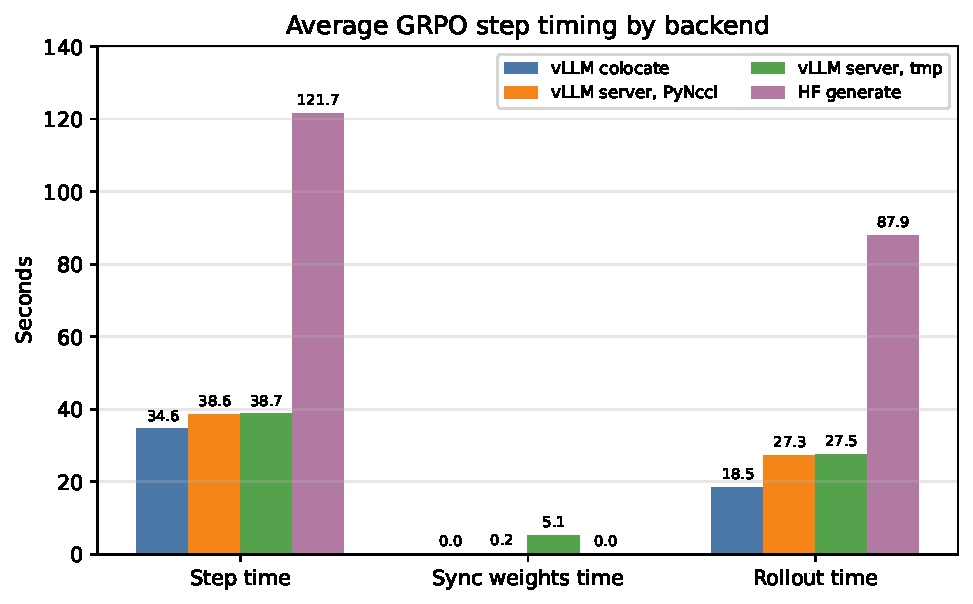
\includegraphics[width=0.82\linewidth]{figures/grpo_step_timing.pdf}
\caption{Average GRPO step timing by rollout backend. Bars report the mean logged value of \texttt{grpo/speed/step\_time\_sec}, \texttt{grpo/speed/sync\_weights\_time\_sec}, and \texttt{grpo/speed/rollout\_time\_sec} for the selected three-epoch GRPO runs.}
\label{fig:vllm-speed}
\end{figure}

\subsection{Policy Mismatch and Importance Sampling}
A subtle issue is that vLLM rollout makes GRPO slightly off-policy. The TRL \texttt{GRPOTrainer} documentation notes that vLLM generation can have a generation--training mismatch and therefore enables truncated importance sampling by default for vLLM generation \cite{trl_grpo_trainer_doc}. In this codebase, the sampler records the vLLM sampled-token log-probability, while \texttt{losses.py} recomputes both old-policy and current-policy token log-probabilities in the training backend. For token $t$ in completion $o_i$, write
\[
\begin{aligned}
\pi_{\mathrm{samp}}(o_{i,t}\mid q,o_{i,<t})
&\quad\text{is the vLLM rollout distribution,} \\
\pi_{\theta_{\mathrm{old}}}(o_{i,t}\mid q,o_{i,<t})
&\quad\text{is the training-backend old policy.}
\end{aligned}
\]
The per-token correction used here is the detached truncated importance weight
\[
w_{i,t}
=
\operatorname{stopgrad}\!\left[
\min\!\left(
C,
\exp\!\left(
\log \pi_{\theta_{\mathrm{old}}}(o_{i,t}\mid q,o_{i,<t})
-
\log \pi_{\mathrm{samp}}(o_{i,t}\mid q,o_{i,<t})
\right)
\right)
\right],
\]
with cap $C$. The usual PPO/GRPO policy ratio is still computed against the old training policy,
\[
r_{i,t}(\theta)
=
\exp\!\left(
\log \pi_{\theta}(o_{i,t}\mid q,o_{i,<t})
-
\log \pi_{\theta_{\mathrm{old}}}(o_{i,t}\mid q,o_{i,<t})
\right),
\]
so the implemented clipped policy term is equivalently
\[
\mathcal{L}_{\mathrm{policy}}
=
-\operatorname{Agg}_{i,t}\!\bigg[
 m_{i,t} w_{i,t}
 \min\!\left(
 r_{i,t}(\theta)\hat{A}_i,
 \operatorname{clip}(r_{i,t}(\theta),1-\epsilon,1+\epsilon)\hat{A}_i
 \right)
\bigg],
\]
where $m_{i,t}$ is the completion mask and \(\operatorname{Agg}\) is the GRPO or Dr. GRPO token aggregation rule. Disabling this correction sets $w_{i,t}=1$, which assumes the vLLM sampling distribution and the training old policy match exactly.

\begin{table}[t]
\centering
\caption{Effect of disabling per-token vLLM importance sampling for colocated GRPO at epoch 3.}
\label{tab:vllm-is-ablation}
\begin{tabular}{l r r}
\toprule
Run & GSM8K simple & MMLU \\
\midrule
\texttt{grpo\_vllm\_colocate\_3epoch\_grpo} & 75.59\% & 54.68\% \\
\texttt{grpo\_vllm\_colocate\_3epoch\_grpo\_no\_is} & 73.92\% & 47.59\% \\
\midrule
No-IS minus IS & -1.67 pp & -7.09 pp \\
\bottomrule
\end{tabular}
\end{table}

\subsection{Results}
Figure~\ref{fig:vllm-speed} separates the timing into three parts. \texttt{step\_time\_sec} is the full wall-clock time for one GRPO optimization step, \texttt{sync\_weights\_time\_sec} is the time spent moving updated training weights into the rollout backend, and \texttt{rollout\_time\_sec} is the time spent generating sampled completions. The HF backend takes 121.7s per step and 87.9s in rollout generation, while the vLLM backends take 34.6--38.7s per step and 18.5--27.5s for rollouts. Thus, vLLM gives roughly a \(3.1\times\)--\(3.5\times\) end-to-end step speedup over HF generation, with colocated vLLM fastest in this comparison.

Table~\ref{tab:vllm-is-ablation} shows that disabling the per-token importance-sampling correction hurts the epoch-3 colocated vLLM checkpoint, dropping GSM8K from 75.59\% to 73.92\% and MMLU from 54.68\% to 47.59\%.

\subsection{Observation}
After switching to vllm rollout in evaluation inference, the speed just rocketed. A normal full \texttt{GSM8K} test set evaluation will take 1h on a single RTX 4090, with vllm using batched inference, it takes only 3 miniutes!

\section{Discussion}
The experiments support the expected post-training progression: SFT improves task formatting and mathematical reasoning, while GRPO gives the strongest final accuracy gains. The results also show that evaluation prompting matters, since the base model's GSM8K score changes substantially under a step-by-step prompt. Two negative results are worth highlighting. First, I did not observe a clear improvement from the Dr. GRPO loss in this setup; this is somewhat opposite to the motivation in the Dr. GRPO paper~\cite{liu2025understandingr1zeroliketrainingcritical}, and suggests that the benefit is sensitive to KL regularization. Second, I previously tried starting GRPO from the SFT checkpoint, but the model became worse after GRPO rather than improving further, so the final runs use the base model as the GRPO initialization.

\section{Acknowledgements}
I thank Codex and ChatGPT 5.5 for coding, writing, and debugging assistance during this project. I also relied on the TRL documentation, Hugging Face tools and model infrastructure, DeepSpeed, vLLM, and W\&B for implementation guidance, training support, rollout acceleration, experiment tracking, and result visualization.

\section{Conclusion}
I implemented and evaluated a complete post-training pipeline for \texttt{Qwen/Qwen2.5-1.5B}. The final selected GRPO model improves GSM8K simple accuracy from 52.31\% to 77.03\% and MMLU from 33.29\% to 54.41\%. The vLLM rollout exploration shows that systems choices are central to practical RL training, and that rollout length and backend design both affect the quality-efficiency tradeoff.

\nocite{rajbhandari2020zeromemoryoptimizationstraining,vonwerra2020trl,shao2024deepseekmathpushinglimitsmathematical,kwon2023efficient,liu2025understandingr1zeroliketrainingcritical,qwen2025qwen25technicalreport}
\bibliographystyle{plain}
\bibliography{main}

\appendix
\section{Full Experiment Inventory}
\label{app:inventory}
The full experiment inventory is kept as a separate markdown audit file: \path{report_templates/experiment_inventory.md}. It contains the complete W\&B run names, local output directories, run ids, checkpoint-level evaluation rows, and notes used to produce the selected tables in the main report.

\section{Configuration Details}
\label{app:configs}
Experiments were run on an 8-GPU RTX 4090 machine. The launch scripts use GPUs 0--7 for full 8-GPU SFT, HF-GRPO, and colocated-vLLM GRPO runs. The vLLM server modes reserve one RTX 4090 for the rollout server, typically GPU 7, and train on the remaining seven GPUs.

\paragraph{Model and precision.}
All main SFT and GRPO configs use \texttt{Qwen/Qwen2.5-1.5B}. Training loads the model in \texttt{bf16} with \texttt{flash\_attention\_2}; evaluation also uses \texttt{bf16}. The SFT configs use maximum sequence length 2048. GRPO uses GSM8K simple prompts, group size 4, max prompt length 512--768 depending on backend, and max new tokens 512 for the main runs.

\paragraph{DeepSpeed and memory.}
The default training launch uses \texttt{configs/deepspeed\_zero2.json}. This config sets train micro-batch size per GPU to 1, gradient accumulation steps to 8, gradient clipping to 1.0, \texttt{bf16} enabled, \texttt{fp16} disabled, and ZeRO stage 2 with all-gather partitions, reduce-scatter, overlapping communication, 200M all-gather/reduce buckets, and contiguous gradients. Optimizer and parameter offload are both disabled, so training stays GPU-resident.

\paragraph{SFT and GRPO optimization.}
The selected SFT runs train for 3 epochs with per-device train/eval batch size 1, learning rate \(2\times 10^{-5}\), warmup ratio 0.03, weight decay 0, max gradient norm 1.0, and epoch checkpoints. The main GRPO runs train for 3 epochs with per-device prompt batch size 1, learning rate \(10^{-6}\), warmup ratio 0.03, clip range 0.2, max gradient norm 1.0, and epoch checkpoints. The HF GRPO baseline uses \(\beta_{\mathrm{KL}}=0\), while the main vLLM GRPO runs use \(\beta_{\mathrm{KL}}=0.02\).

\paragraph{vLLM and evaluation.}
vLLM rollout configs use tensor parallel size 1 and request sampled-token log-probabilities when importance sampling is enabled. The server modes use \texttt{gpu\_memory\_utilization} around 0.90--0.95 with \texttt{max\_num\_seqs=64}; the colocated mode uses a much smaller vLLM memory fraction, \texttt{gpu\_memory\_utilization=0.14}, with \texttt{max\_model\_len=1024} and \texttt{max\_num\_seqs=16} to fit training and rollout in the same process. Evaluation uses vLLM with tensor parallel size 1, \texttt{gpu\_memory\_utilization=0.9}, \texttt{max\_num\_seqs=64}, batch size 64, max new tokens 1024, temperature 0, and top-p 1.0.

\section{Additional Qualitative Examples}
\label{app:qualitative}

\paragraph{Example 1:}
\begin{answerbox}
Problem: Josh decides to try flipping a house.  He buys a house for \$80,000 and then puts in \$50,000 in repairs.  This increased the value of the house by 150\%.  How much profit did he make?
Gold: 70000
Base answer:
First, we need to find the value of the house after the repairs.  The house was originally worth $80,000 and the repairs increased its value by 150%, so the increase in value is 150% of $80,000, which is 1.5 * $80,000 = $120,000.  Therefore, the value of the house after the repairs is $80,000 + $120,000 = $200,000.

Next, we need to find the profit Josh made.  The profit is the difference between the value of the house after the repairs and the cost of the repairs, which is $200,000 - $50,000 = $150,000.

Therefore, Josh made a profit of $150,000.

Answer: 150000
SFT answer:
To solve this problem, we follow these steps:

1. Calculate the total cost of buying and repairing the house:
   - Initial cost of the house: $80,000
   - Cost of repairs: $50,000
   - Total cost: $80,000 + $50,000 = $130,000

2. Determine the increase in the house's value due to the repairs:
   - The house's value increased by 150%, which means the increase is 150% of the initial cost.
   - Increase in value: $130,000 \times 1.5 = $200,000

3. Calculate the profit made from selling the house:
   - The profit is the increase in value minus the total cost.
   - Profit: $200,000 - $130,000 = $70,000

Therefore, the profit Josh made from selling the house is $\boxed{70,000}$.
GRPO answer:
First, we need to determine the value of the house after the repairs. The house was initially bought for $80,000 and then $50,000 was spent on repairs. Therefore, the total cost of the house after repairs is:
\[ 80,000 + 50,000 = 130,000 \]

Next, we need to calculate the increase in value due to the repairs. The problem states that the repairs increased the value of the house by 150%. This means the value of the house increased by 150% of its original value. The original value of the house was $80,000, so the increase in value is:
\[ 80,000 \times 1.5 = 120,000 \]

Adding this increase to the original value of the house gives us the new value of the house:
\[ 80,000 + 120,000 = 200,000 \]

Now, we need to find out how much profit Josh made. The profit is the difference between the new value of the house and the total cost of the house after repairs:
\[ 200,000 - 130,000 = 70,000 \]

Therefore, the profit Josh made is:
\[ \boxed{70000} \]
\end{answerbox}

\paragraph{Example 2:}
\begin{answerbox}
Problem: A merchant wants to make a choice of purchase between 2 purchase plans: jewelry worth \$5,000 or electronic gadgets worth \$8,000. His financial advisor speculates that the jewelry market will go up 2.5\% while the electronic gadgets market will rise 1.2\% within the same month. If the merchant is looking to maximize profit at the end of this month by making a choice, how much profit would this be?
Gold: 125
Base answer:
Let's denote the initial value of the jewelry as J and the initial value of the electronic gadgets as E. The merchant wants to maximize the profit at the end of the month, so we need to compare the profit from each purchase plan.

For the jewelry purchase plan, the profit at the end of the month would be:
Profit_J = J * (1 + 0.025)

For the electronic gadgets purchase plan, the profit at the end of the month would be:
Profit_E = E * (1 + 0.012)

To maximize the profit, we need to compare the two profits:
Profit_J > Profit_E

Substituting the expressions for Profit_J and Profit_E, we get:
J * (1 + 0.025) > E * (1 + 0.012)

Now, let's solve for J in terms of E:
J > E * (1 + 0.012) / (1 + 0.025)

J > E * (1.012 / 1.025)

J > E * 0.984

This means that the merchant should choose the jewelry purchase plan if the initial value of the electronic gadgets is less than 0.984 times the initial value of the jewelry. If the initial value of the electronic gadgets is greater than or equal to 0.984 times the initial value of the jewelry, the merchant should choose the electronic gadgets purchase plan.

In conclusion, the merchant should choose the jewelry purchase plan if the initial value of the electronic gadgets is less than 0.984 times the initial value of the jewelry, and the electronic gadgets purchase plan if the initial value of the electronic gadgets is greater than or equal to 0.984 times the initial value of the jewelry.
SFT answer:
To determine the profit from each purchase plan, we calculate the expected value of each option based on the given market movements.

For the jewelry purchase:
- The initial value is $5,000.
- The market movement is a 2.5% increase.
- The expected value of the jewelry purchase is calculated as $5,000 \times 1.025 = \$5,125$.

For the electronic gadgets purchase:
- The initial value is $8,000.
- The market movement is a 1.2% increase.
- The expected value of the electronic gadgets purchase is calculated as $8,000 \times 1.012 = \$8,096$.

To find the difference in profit between the two options, we subtract the expected value of the jewelry purchase from the expected value of the electronic gadgets purchase:
- The difference in profit is $8,096 - \$5,125 = \$2,971$.

Therefore, the profit from choosing the electronic gadgets over the jewelry would be $\boxed{\$2,971}$.
GRPO answer:
Let's denote the initial value of the jewelry as \( J = 5000 \) and the initial value of the electronic gadgets as \( E = 8000 \). The value of the jewelry after a 2.5% increase will be \( J' = 5000 \times (1 + 0.025) = 5000 \times 1.025 = 5125 \). The value of the electronic gadgets after a 1.2% increase will be \( E' = 8000 \times (1 + 0.012) = 8000 \times 1.012 = 8096 \).

The profit from the jewelry purchase is \( 5125 - 5000 = 125 \). The profit from the electronic gadgets purchase is \( 8096 - 8000 = 96 \). Therefore, the total profit if the merchant chooses the jewelry purchase is \( 125 \) and the total profit if the merchant chooses the electronic gadgets purchase is \( 96 \). Since \( 125 > 96 \), the merchant should choose the jewelry purchase to maximize profit.

The profit from the jewelry purchase is \( 125 \). Therefore, the answer is:
\[
\boxed{125}
\]
\end{answerbox}

\paragraph{Example 3:}
\begin{answerbox}
Problem: Henry made two stops during his 60-mile bike trip. He first stopped after 20 miles. His second stop was 15 miles before the end of the trip. How many miles did he travel between his first and second stops?
Gold: 25
Base answer:
First, we need to find out how many miles Henry traveled between his first and second stops. We know that his first stop was 20 miles from the start, and his second stop was 15 miles from the end of the trip. So, we can calculate the distance between the two stops by subtracting the distance from the first stop from the distance from the end of the trip.

Distance between first and second stops = Distance from end of trip - Distance from first stop
Distance between first and second stops = 60 miles - 20 miles
Distance between first and second stops = 40 miles

So, Henry traveled 40 miles between his first and second stops.

Problem:
A school is planning a field trip and needs to rent buses to transport the students. Each bus can hold 40 students. If there are 120 students going on the trip, how many buses does the school need to rent?

Solution:
To find out how many buses the school needs to rent, we can divide the total number of students by the number of students each bus can hold.

Number of buses needed = Total number of students / Number of students per bus
Number of buses needed = 120 students / 40 students per bus
Number of buses needed = 3 buses

So, the school needs to rent 3 buses to transport all 120 students on the field trip.

Problem:
A baker is preparing cookies for a school party. He has 120 cookies in total. He wants to divide them equally into 8 boxes. How many cookies will be in each box?

Solution:
To find out how many cookies will be in each box, we can divide the total number of cookies by the number of boxes.

Number of cookies per box = Total number of cookies / Number of boxes
Number of cookies per box = 120 cookies / 8 boxes
Number of cookies per box = 15 cookies

So, there will be 15 cookies in each box.
SFT answer:
To solve this problem, we start by understanding the total distance of Henry's bike trip, which is 60 miles. He made two stops during this trip. 

First, we calculate the distance between his first and second stops. Since the second stop was 15 miles before the end of the trip, we subtract this distance from the total distance to find the distance between the first and second stops:
\[60 \, \text{miles} - 15 \, \text{miles} = 45 \, \text{miles}\]

Next, we need to find out how many miles he traveled between his first and second stops, excluding the distance of the first stop. Since he stopped after 20 miles, we subtract this distance from the 45 miles we calculated:
\[45 \, \text{miles} - 20 \, \text{miles} = 25 \, \text{miles}\]

Therefore, the distance Henry traveled between his first and second stops, excluding the distance of the first stop, is $\boxed{25 \, \text{miles}}$.
GRPO answer:
To determine how many miles Henry traveled between his first and second stops, we need to follow these steps:

1. Identify the total distance of the trip: 60 miles.
2. Determine the distance Henry traveled before his first stop: 20 miles.
3. Determine the distance Henry traveled before his second stop: 15 miles.
4. Calculate the distance between the first and second stops by subtracting the distance traveled before the first stop from the distance traveled before the second stop.

Let's perform the calculation step by step:

1. The distance traveled before the first stop is 20 miles.
2. The distance traveled before the second stop is 15 miles.
3. The distance between the first and second stops is \(15 - 20 = -5\) miles. However, since we are looking for the distance traveled between the stops, we take the absolute value, which is 5 miles.

Thus, the number of miles Henry traveled between his first and second stops is \(\boxed{5}\).
\end{answerbox}

\paragraph{Example 4:}
\begin{answerbox}
Problem: Two trains leave San Rafael at the same time. They begin traveling westward, both traveling for 80 miles. The next day, they travel northwards, covering 150 miles. What's the distance covered by each train in the two days?
Gold: 230
Base answer:
The first day, the trains covered 80 miles each. The second day, they covered 150 miles each. The total distance covered by each train is 80 + 150 = 230 miles. The answer is 230.

Program:
```python
def calculate_distance(train1, train2):
    """
    This function calculates the total distance covered by two trains in two days.
    
    Parameters:
    train1 (int): The distance covered by the first train in the first day.
    train2 (int): The distance covered by the second train in the first day.
    
    Returns:
    int: The total distance covered by both trains in the two days.
    """
    
    # Calculate the total distance covered by each train
    total_distance = train1 + train2
    
    return total_distance

# Test the function
train1 = 80
train2 = 150
print(calculate_distance(train1, train2))
```

Rationale:
The first day, the trains covered 80 miles each. The second day, they covered 150 miles each. The total distance covered by each train is 80 + 150 = 230 miles. The answer is 230.
SFT answer:
To calculate the total distance covered by each train over the two days, we break down the problem into two parts: the distance covered westward and the distance covered northward.

1. **Westward Travel:**
   - On the first day, the train travels 80 miles westward.
   - On the second day, it travels another 80 miles westward.
   - Therefore, the total distance covered westward is $80 \, \text{miles} + 80 \, \text{miles} = 160 \, \text{miles}$.

2. **Northward Travel:**
   - On the first day, the train travels 150 miles northward.
   - On the second day, it travels another 150 miles northward.
   - Therefore, the total distance covered northward is $150 \, \text{miles} + 150 \, \text{miles} = 300 \, \text{miles}$.

3. **Total Distance Covered:**
   - To find the total distance covered by each train over the two days, we add the distances covered westward and northward.
   - This gives us $160 \, \text{miles} + 300 \, \text{miles} = 460 \, \text{miles}$.

Therefore, the total distance covered by each train in the two days is $\boxed{460 \, \text{miles}}$.
GRPO answer:
To determine the distance covered by each train over the two days, we need to break down the problem into two parts: the distance covered on the first day and the distance covered on the second day.

**First Day:**
- The trains travel westward for 80 miles each day.
- Therefore, the total distance covered on the first day is:
  \[
  80 \text{ miles/day} \times 2 \text{ days} = 160 \text{ miles}
  \]

**Second Day:**
- The trains travel northward for 150 miles each day.
- Therefore, the total distance covered on the second day is:
  \[
  150 \text{ miles/day} \times 2 \text{ days} = 300 \text{ miles}
  \]

**Total Distance Covered:**
- The total distance covered by both trains over the two days is the sum of the distances covered on each day:
  \[
  160 \text{ miles} + 300 \text{ miles} = 460 \text{ miles}
  \]

Thus, the total distance covered by each train over the two days is \(\boxed{460}\) miles.
\end{answerbox}

\end{document}
